\chapter{Statistica descrittiva}

Il corso tratterà tre principali argomenti: \textbf{statistica descrittiva}, \textbf{probabilità} e
\textbf{inferenza statistica}.

Questa prima parte di \emph{statistica descrittiva} tratterà l'analisi di dati senza la costruzione di un
modello d'interpretazione.

Due dei concetti preliminari e fondamentali sono quelli di \textbf{popolazione} e \textbf{campione}:
\begin{itemize}
	\item \textbf{Popolazione}: cardinalità dell'insieme che stiamo considerando.
	\item \textbf{Campione}: cardinalità di un sottoinsieme più piccolo dell'insieme che stiamo considerando.
\end{itemize}

\begin{example}
	Gli italiani che hanno partecipato alle ultime votazioni (45 milioni circa) sono una \emph{popolazione}.
	Quando si fa un sondaggio elettorale si prende in considerazione un \emph{campione} della popolazione (per
	esempio qualche migliaio di votanti).
\end{example}

Altri due concetti di base sono quelli di \textbf{frequenza assoluta} e \textbf{frequenza relativa}:
\begin{itemize}
	\item \textbf{Frequenza assoluta}: il valore assoluto con il quale occorre un certo valore.
	\item \textbf{Frequenza relativa}: la percentuale con la quale un certo valore compare all'interno
	      dell'insieme dell'insieme considerato.
\end{itemize}

\begin{example}
	Se un candidato sindaco prende 1234 voti su 6342 votanti allora 1234 è la \emph{frequenza assoluta} del
	suo voto. La frequenza relativa si calcola banalmente:
	\[ \frac{1234}{6342} = 0.194 \]
	dunque $0.194$ è la \emph{frequenza relativa} del voto, ossia il $19.4 \%$ dei voti.
\end{example}

\section{Rappresentazione grafica delle frequenze}
In statistica si farà spesso uso di rappresentazioni grafiche di vario genere come diagrammi a torta, istogrammi
ecc.

\begin{example}
	Per esempio se volessimo analizzare quanti studenti, iscritti all'università di Pisa sono pisani, quanti sono
	toscani e quanti provengono da fuori della Toscana possiamo usare un grafo a torta.
	\begin{center}
		\begin{tikzpicture}[scale=0.5]
			\pie[color = { yellow!70, red!70, blue!70 }] {
				40/Pisa,
				25/Toscana,
				45/Altro
			}
		\end{tikzpicture}
	\end{center}
\end{example}

\begin{example}
	Altra rappresentazione molto utilizzata è quella tramite istogrammi, per esempio per rappresentare quante famiglie
	hanno un determinato numero di figli in una certa zona.
	\begin{center}
		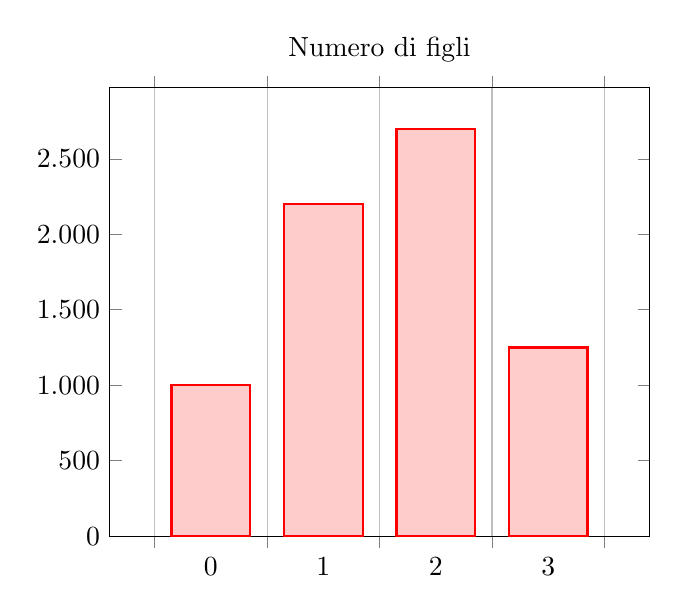
\begin{tikzpicture}
			\begin{axis}[
					title = {Numero di figli},
					y tick label style={/pgf/number format/use comma},
					ybar,
					ybar interval = 0.7,
					ymin = 0
				]

				\addplot [
					thick,
					draw=red,
					fill=red!20
				]
				coordinates {(0, 1000) (1, 2200) (2, 2700) (3, 1250) (4, 10)};
			\end{axis}
		\end{tikzpicture}
	\end{center}
\end{example}